% !TEX root = ../main.tex
\section{Representability Diagnostics in Truncated Baths}
\label{sec:numerical_results}

The physical-regime diagnostics above identify where the exact reduced state
changes most rapidly. We now ask how finite-basis numerics behave across that
same region. The exact qubit solution developed in the previous section depends
on the bath only through response data at three frequencies,
\(\omega\in\{0,\pm\omega_q\}\). To test it we
compare against exact diagonalization (ED) of a truncated spin-boson model,
where the qubit is coupled to \(N_\omega\) harmonic oscillators and each mode
is represented with a finite Fock cutoff \(n_{\max}\). A useful feature of this
comparison is that the analytic kernel integrals can be evaluated in two ways:
using the full continuum spectral density (the \emph{continuous analytic}
branch) or using the same discrete mode set seen by ED (the \emph{discrete
analytic} branch). The comparison therefore tests not only the exact reduced
generator but also whether a chosen finite numerical representation can realize
the same compact reduced description.

Figure~\ref{fig:ed_vs_analytic} compares the excited-state population
\(p_{11}\) across coupling strengths and inverse temperatures for
\(N_\omega=40\) modes. At small \(\chi\), all three curves coincide. As the
system crosses the exact response scale \(\chi\sim 1\), the analytic
predictions separate from ED. The key point is that the discrete analytic
branch does \emph{not} follow the numerical deviation: it bends back toward the
continuum benchmark. This shows that the exact HMF theory is already correct
for the discrete mode set itself. The discrepancy is therefore not a failure of
the theory, nor a finite-mode artifact.

The remaining gap is a representability bottleneck in the truncated Hilbert
space. In the large-response regime the coupled system approaches a displaced,
polaron-like ground state, and faithfully representing that state requires
\(n_{\max}\gtrsim |\alpha_k|^2\) for each displaced mode
\(\alpha_k\sim g_k/\omega_k\). Once \(\chi\gtrsim 1\), the chosen Fock cutoff
can no longer support the required occupations. ED is then trapped in a model
class that is too small to contain the exact dressed equilibrium state. In the
language of the compositional discussion above, the target reduced generator is
known exactly but the chosen finite representation lacks the capacity to
realize it.

\begin{figure}[t]
  \centering
  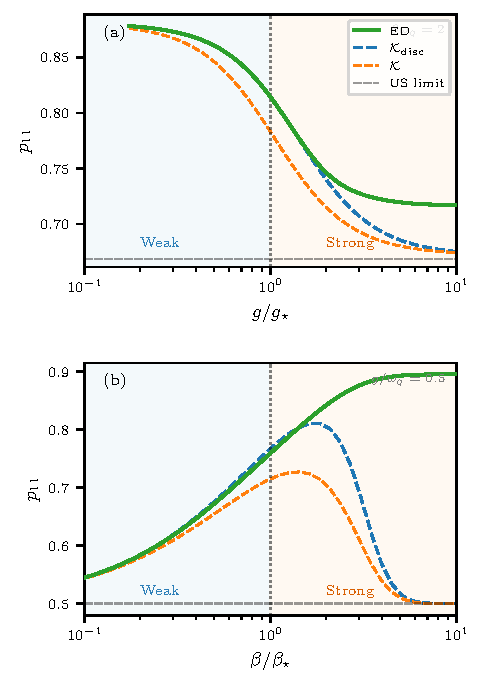
\includegraphics[width=0.48\textwidth]{../figures/hmf_fig2_ed_vs_analytic.pdf}
  \caption{Excited-state population \(p_{11}\) across the exact response scale
    for \(N_\omega=40\) modes. Green solid: ED. Blue dashed: discrete analytic
    theory using the same mode set. Orange dotted: continuum analytic theory.
    Dashed horizontal lines mark the large-response benchmark \(p_\infty\). The
    gap between ED and the analytic branches is a representability failure of
    the truncated basis, not a breakdown of the exact reduced generator.}
  \label{fig:ed_vs_analytic}
\end{figure}

The same interpretation explains the bandwidth sensitivity in
Fig.~\ref{fig:bandwidth_convergence}. Varying the spectral window changes how
the displacement load is distributed over the available modes. As the system is
pushed across the response scale, the required occupations grow and the
available Fock space is exhausted. The sharp peak in cutoff sensitivity is
therefore a direct signature of the finite basis hitting its representational
boundary.

\begin{figure}[t]
  \centering
  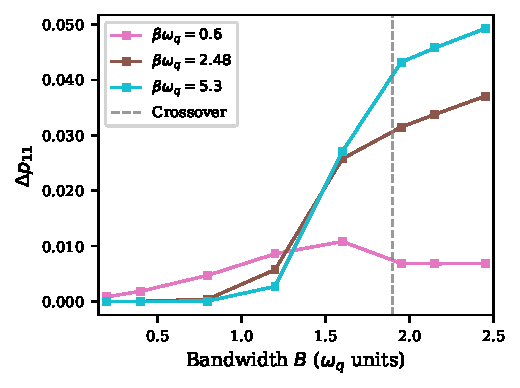
\includegraphics[width=0.48\textwidth]{../figures/hmf_fig3_bandwidth_convergence.pdf}
  \caption{Cutoff sensitivity
    \(\Delta p_{11}\equiv |p_{11}(n_{\max}=4)-p_{11}(n_{\max}=6)|\) as a
    function of spectral bandwidth \(B\) in units of \(\omega_q\). The
    sensitivity peak marks the onset of the representability bottleneck: beyond
    this point the truncated basis can no longer accommodate the mode
    occupations required by the exact dressed state.}
  \label{fig:bandwidth_convergence}
\end{figure}

The numerical message is therefore narrower, and stronger, than a generic
``agreement with simulation'' claim. The analytic HMF provides the correct
reduced target for both discrete and continuous baths. The observed numerical
deviations diagnose when a chosen finite model class is no longer expressive
enough to realize that target.
